\documentclass[12pt,oneside]{memoir} 
\usepackage[latinica]{matfmaster}
\usepackage[latinica]{pangrami}
\usepackage{mathtools}
\usepackage{amsmath}
\usepackage{amsthm}
%\usepackage{fixltx2e} %kod mene ne treba ovaj paket
\usepackage{graphicx}
\usepackage{url}


% Datoteka sa literaturom u BibTex tj. BibLaTeX/Biber formatu
%\bib{Master_rad}

\autor{Ljubica Peleksić}
\naslov{Klasifikacija obolelih od Alchajmerove bolesti na osnovu analize spontanog govora}
\godina{2021}

\mentor{doc. dr Jelena Graovac, profesor\\ Univerzitet u Beogradu, Matematički fakultet}

% Dodati clanove komisije i datum odbrane
\komisijaA{prof. dr Gordana Pavlović-Lažetić}
\komisijaB{doc. dr Jovana Kovačević}
\datumodbrane{}

% Apstrakt na srpskom jeziku (u odabranom pismu)
\apstr{%
% TODO Dodati apstrakt
}



% Ključne reči na srpskom jeziku (u odabranom pismu)
\kljucnereci{klasifikacija, Alchajmer, NLP}

\begin{document}

% ==============================================================================
% Uvodni deo teze
\frontmatter
% ==============================================================================
% Naslovna strana
\naslovna
% Strana sa podacima o mentoru i članovima komisije
\komisija
% Strana sa posvetom (u odabranom pismu)
% TODO Dodati posvetu
\posveta{porodici}
% Strana sa podacima o disertaciji na srpskom jeziku
\setsecnumdepth{subsection}

% Sadržaj teze
\tableofcontents{}

% ==============================================================================
% Glavni deo teze
\mainmatter
% ==============================================================================

% ------------------------------------------------------------------------------

\chapter{Uvod}

Alchajmerova bolest je najčešći oblik demencije koja uzrokuje probleme sa pamćenjem, mišljenjem, govorom i ponašanjem. Simptomi se obično razvijaju polako i vremenom se pogoršavaju do te mere da obolelim osobama znatno mogu ometati obavljanje svakodnevnih zadataka. Dešavaju se kada su neuroni u delovima mozga koji su zaduženi za učenje i memoriju, tj. kognitivne funkcije oštećeni \cite{Alzheimerfactsfigures}. Jedan od najranijih simptoma je otežano pamćenje novih informacija, a zatim nastupaju poteškoće u govoru i gubitak memorije. Kasnije u toku bolesti se pojavljuju i problemi pri obavljaju nekih jednostavih zadataka, gubitak sposobnosti da nastave razgovor i da reaguju na svoju okolinu, vremenska i prostorna dezorijentacija. Alchajmerova bolest ne predstavlja normalan deo starenja iako godine predstavljaju najizraženiji faktor rizika. Oko 6\% do 10\% ljudi preko 65 godina ima neki oblik demencije, a 60\% do 70\% tih ljudi ima upravo Alchajmerovu bolest \cite{actavis}. Svake tri sekunde u svetu neko razvije demenciju, a Alchajmerova bolest je najčešći oblik demencije. Procenjuje se da danas oko 50 miliona ljudi u svetu ima Alchajmerovu bolest ili demenciju vezanu za nju. Pretpostavlja se da bi ovaj broj mogao da naraste do 82 miliona do 2030. godine, a do 152 miliona do 2050. godine \cite{Languageimpairment}. U proseku, osoba sa Alchajmerovom bolešću živi četiri do osam godina nakon dijagnoze, ali može da živi i do 20 godina, u zavisnosti od drugih faktora \cite{seracell}.

Tačan uzrok bolesti nije poznat, ali se pretpostavlja da učestvuje više udruženih faktora kao što su genetski činioci, ranija oboljenja, uticaj životne sredine i promene na mozgu uzrokovane starenjem \cite{medicor}.

Metodi za dijagnostifikovanje bolesti se sastoje iz struktuiranih intervjua koje izvode lekari. Tokom ovih intervjua teško je da se uoči kompleksna priroda nedostataka koji se mogu naći u govoru obolele osobe.

Ovi intervjui testiraju jezičke sposobnosti i uključuju imenovanje objekata, izgovaranje jedne reči, generisanje reči iz datog konteksta ili generisanje reči sa određenim početnim slovom \cite{automaticdetandrat}. Dijagnostifikovanje Alchajmerove bolesti je najlakše iz ugla porodice i prijatelja, pošto su oni u stanju da u svakodnevnom životu, pri normalim konverzacijama, primete male promene u ponašanju bližnjih.

Teži se automatizovanom pristupu sa objektivnim metodama dijanostifikovanja bolesti, kao i određivanja stepena progresije. Ovakav novi pristup je neophodan kako zbog preciznosti i zbog ranog dijagnostifikovanja bolesti, tako i zbog brzine dobijanja dijagnoze i činjenice da bi time dijanozu i tretman za ublažavanje simptoma moglo dobiti više ljudi u svetu, među kojima danas mnogi nemaju pristup lekarima i lekarskoj nezi. Takođe, ovo bi omogućilo dijagnozu osobama sa izrazito napredom demencijom koje ne mogu da prolaze kroz psihološko testiranje. Takođe, automatizovan pristup bi doneo i mogućnost da se odredi nivo poboljšanja kod obolelog u toku ili nakon neke terapije ili leka \cite{Evaloftechfolexicalperformance}.

Zato tražimo metod za dijanostifikovanje koji je pouzdan, objektivan, lak za izvođenje i dovoljno precizan.

Prema Svetskom izvestaju o Alchajmeru iz 2011. godine postoje benefiti rane dijagnoze i intervencije koji su efektivniji u ranim stadijumima bolesti i omogućava osobama da isplaniraju negu i tretmane koje žele da imaju u budućnosti. Pored korišćenja lekova, a ima ih nekoliko, smanjenje pogoršanja kognitivnih funkcija osobe može pružiti i specijalizovana terapija.

U više naučnih radova i studija je pokazano da korišćenjem obrade prirodnog jezika (eng. natural language processing) i mašinskog učenja (eng. machine learning) se može doći do vrednih podataka. Motivacija za ovom vrstom obrade podataka i zaključivanja, koji će biti predstavljeni u narednim poglavljima, je nastala iz \cite{automaticdetandrat} i \cite{linguisticfeatures}.

Problem koji se rešava u okviru ovog rada je da li je moguće primeniti automatizaciju postupka dijagnostifikovanja obolelih od Alchajmerove bolesti dovoljno precizno, tačnije, da li je moguće razlikovati starije subjekte od subjekata koji pate od Alchajmerove bolesti na osnovu spontanog govora. Ono što pojedinac izgovara je nepresušan izvor informacija o njemu samom, a upravo tom činjenicom se vodimo kada vidimo mogućnost u nalaženju dijanoze analizom spontanog govora. Dva pravca istraživanja su praćena, jedan lingvistički i drugi putem metoda mašinskog učenja. U sklopu lingvističkog pristupa,  određene, već poznate metrike se izračunavaju za svaki intervju, koji je predstavljen skupom reči, njenom vrstom reči i lemom. U okviru ovog pristupa tražimo pravilnosti u govoru koje nam mogu pokazati da osoba boluje baš od ove bolesti. U pristupu mašinskim učenjem ne postoje poznate metrike, već se prepušta algoritmima da uoče zakonitosti u podacima u obliku učestalosti korišćenja reči i na taj način se preciziraju zakonitosti i razlike između dve grupe pacijenata.

Do danas nije pronađen lek koji zaustavlja ili usporava razvoj bolesti, ali postoje lekovi za koje se smatra da mogu da uspore bolest ako je rano dijagnostifikovana, kao i oni za koje se smatra da poboljšavaju kognitivne funkcije obolele osobe \cite{Alzheimerfactsfigures}. Lekovi za demenciju mogu da uspore napredovanje bolesti u ranim i srednjim fazama.  Cilj lečenja Alchajmerove bolesti je što duže očuvanje sposobnosti i samostalnosti bolesnika. Osim redovnog uzimanja lekova značajna je i primena drugih mera koje mogu u velikoj meri pomoći pacijentu \cite{medicor}.

Ovu temu razrađujemo kroz šest poglavlja, gde se nakon uvodnog poglavlja osvrćemo na podatke korišćene u praktičnom radu, način prikupljanja i obrade podataka. U drugom poglavlju je opisan način rešavanja ovog problema metodama lingvističke analize, gde su predstavljene metrike koje su korišćene kao i motivacija za njihov izbor. Treće poglavlje predstavlja prikaz rešavanja problema metodama mašinskog učenja, modele reprezentacije teksta kao i algoritme mašinskog učenja koji su iskorišćeni u praktičnom radu. U okviru petog poglavlja se diskutuju dobijeni rezultati reprezentativnog uzorka, primenama svih metoda, dok se u poslednjem poglavlju, u okviru zaključka, sumiraju dobijeni rezultati i korišćene metode.

\chapter{Podaci}

Kod rešavanja problema obradom prirodnih jezika, pored važnosti algoritama koji se koriste, treba istaći važnost podataka koji se koriste u tim algoritmima.  Bez podataka, algoritam sam nema nikavu vrednost.  Izazov je, sam po sebi, pronaći dovoljnu količinu podataka, kao i da oni imaju potreban kvalitet, da bi eksperimenti bili uspešni.  U slučaju klasifikacije obolelih od Alchajmerove bolesti bilo je neophodno prikupiti intervjue sa obolelim ljudima od ove bolesti, kao i intervjue sa nedementnim starijim osobama. Zatim, bilo je neophodno napraviti transkripte tih intervjua, kako bi se dobili ulazni podaci u tekstualnom formatu pogodnom za obradu od strane kreiranih algoritama. Zahvaljujući pojedincima i grupi volontera sa Biološkog fakulteta u Beogradu, ali i intervjuisanim osobama koje su pristale da izdvoje vreme i budu intervjuisane, dobijen je skup podataka neprocenjive vrednosti i oni će biti korišćeni u ovom radu.

Podaci korišćeni za rešavanje problema klasifikacije obolelih osoba od Alchajmerove bolesti su transkripti slobodnog govora osoba. Transkripti su prikupljeni kao audio ili video zapisi, a razgovori sa osobama nisu strukturirani niti imaju neki određeni sled. Osoba se ohrabruje da priča o sebi i svom životu, kao i o bližnjima. Na osobi koja intervjuiše je da postavlja pitanja, dok intervjuisani odgovara. Osoba koja intervjuiše takođe prati tok razgovora sa pitanjima, te nisu u svakom razgovoru ista.

U cilju rešavanja klasifikacije, dve grupe ispitanika su intervjuisane: oboleli od Alchamjera i starije nedementne osobe kod kojih nije dijanostifikovana ova bolest.

Intervjui sa osobama obolelim od Alchajmera su sakupljani u obliku video i audio zapisa koji su prikupljeni od osoba koje su koristile usluge dnevnog boravka za obolele od Alchajmera u Novom Sadu, jedine takve ustanove u Srbiji organizovane od strane Udruženja građana Alchajmer. Ovi intervjui su bili prikpljani tokom grupnih razgovora sa obolelima. Intervjui sa nedementnim starijim osobama su prikupljeni i zapisani zahvaljujući aktivnostima više od 20 volontera studenata Biološkog fakulteta u Beogradu, krajem 2017. godine i u toku 2018. godine.

Od audio zapisa razgovora sa osobama su kreirani transkripti. Svaki intervju je zapisan na dva načina: prvi, kao originalan, u kome je svaka reč napisana tačno onako kako je izgovorena, uključujući ponavljanja, nedovršene reči, greške u izgovoru i drugi u kome su ispravljene sve greške u izgovoru. Prvi,je razvijen za potrebe primene metoda mašinskog učenja, a drugi, kako bismo bili u mogućnosti da primenimo metode lingvističke analize teksta. Kako su ovi intervjui sprovedeni grupno, prvi korak je bio da se razdvoje razgovori, tako da rečenice koje je izgovorila jedna osoba se nalaze u jednoj tekstualnoj datoteci koja nosi ime te osobe. U okviru datoteke se nalaze samo reči koje je izgovorila upravo ta osoba. Datoteka nosi ime osobe i ona je u \textit{txt} formatu.  Reci koje je izgovorila osoba koja intervjuise i postavlja pitanja se ne nalaze u datoteci i ne predstavljaju podatke koji se obradjuju. Nakon toga transkripti su pažljivo obrađeni, tako da svaki bude ispravno podeljen na rečenice. Ovaj korak je bio veoma važan kako bi primenom metoda obrade prirodnih jezika mogla ispravno da se izvrši lematizacija, da se odrede vrste reči i da se na pravi način tekst pripremi za dalju obradu.

Transkripti su zapisivani po definisanom protokolu koji se, između ostalog, sastoji iz sledećih pravila:

\begin{enumerate}
\item Intervju sa jednom osobom se nalazi u datoteci koja nosi ime te osobe
\item Ime obolelog se označava vitičastim zagradama
\item Pitanje postavljeno od strane osobe koja vodi intervju se označava uglastim zagradama
\item Koristi se UFT-8 kodna šema i latinica
\item Koriste se slova sa dijakriticima (č, ć, š, đ...)
\item Pauze između izgovorenih reči se zapisuju odgovarajućim brojem crtica, gde svaka crtica predstavlja jedan sekund pauze
\item Brojevi se zapisuju sa crticom između, ako su višecifreni brojevi
\end{enumerate}
i tako dalje.  

Nakon što su transkripti bili ispravno zapisani po protokolu, a rečenice ispravno podeljene, odbačena su pitanja osobe koja intervjuiše, ime obolelog koje se pojavljuje pre početka njegovog odgovora, kao i svi komentari. U datoteci ostaju samo reči koje je intervjuisana osoba izgovorila. Takve datoteke su prosleđene programu gde je algoritamskim putem za svaku reč određena vrsta reči i njena lema. Vrste reči biće upotrebljene u okviru rešavanja problema klasifikacije obolelih od Alchajmerove bolesti lingvističkim metodama. Lema reči se koristi pri računanju vrednosti vokabulara i vokabulara za reči izgovorene jednom. Ove metrike će biti pomenute u daljem radu, u sekciji koja se bavi rešavanjem problema metodama lingvističke analize.

\section{Problem određivanja vrsta reči}

Problem određivanja vrsta reči za reči koje se pojavljuju u tekstu je uobičajen problem u procesiranju prirodnog jezika (eng. Natrual Language processing) i naziva Part-of-Speech-tagging (Pos-tagging).  Programi koji izvršavaju ovaj zadatak se nazivaju tagerima (eng. taggers).  Metoda određivnja vrsta reči je kompleksan problem, ali bitan i izazovan. Posebno težak problem jeste kreiranje ovakvog programa na srpskom jeziku, zbog prirode jezika kao i male količine resursa.  Uz problem određivanja vrsta reči, često se rešava i problem lematizacije, tačnije pridavanje leme reči. Vrste reči koje postoje i njihove oznake na engleskom jeziku su sledece:

\begin{enumerate}
\item Pridev: ADJ
\item Apozicija: ADP
\item Prilog: ADV
\item Pomoćni: AUX
\item Veznici: CCONJ
\item Član: DET
\item Uzvik: INTJ
\item Imenica: NOUN
\item Broj: NUM
\item Rečca: PART
\item Zamenica: PRON
\item Vlastita imenica: PROPN
\item Znak interpunkcije: PUNCT
\item Veznik: SCONJ
\item Simbol: SYM
\item Glagol: VERB
\item Drugo: X
\end{enumerate}

Zadatak je takav da dodeljujemo svakoj reči $x_i$ u ulaznoj sekvenci reči labelu $y_i$, tako da izlazna sekvenca Y ima istu dužinu kao ulazna sekvenca X \cite{postagging}. Reči imaju više mogućih vrsta reči i zadatak ovog procesa je da se pronađe ispravna vrsta reči za svaku pojedinu situaciju. Za reči se određuje takva vrsta koja je najverovatnija. Za mnoge je verovatnoća da pripadaju svim vrstama osim jednoj izuzetno mala, pa je lako odlučiti se.

Jedan od načina da se reši problem određivanja vrsta reči je da se koristi Skriveni Markovljev model (eng. Hidden Markov Model / HMM). Skriveni Markovljev model je probabilistički sekvencijalni model koji za sekvencu jedinica izračunava raspodelu verovatnoće po mogućim sekvencama i bira najbolju opciju. Markovljev lanac, model koji nam govori o verovatnoćama sekvenci slučajnih promenljivih, ima pretpostavku da ako želimo da predvidimo buduće stanje, jedino što je bitno je trenutno stanje. Markovljev lanac se grafički predstavlja grafom, gde su čvorovi grafa stanja, a grane predstavljaju verovatnoće. Suma svih vrednosti grana koje idu iz određenog čvora mora biti jedan. Markovljev lanac se oslanja na događaje koji mogu da se posmatraju, dok u slučaju reči to nije moguće. Zato se koriste Skriveni Markovljev Modeli, koji poseduje skrivene promenljive. Zadatak određivanja skrivene sekvence promenljivih na osnovu observacija u modelu se naziva dekodiranje. Skriveni Markovljev Model počiva na dve pretpostavke. Prva je identična kao za Markovljev lanac, dok druga kaže da verovatnoća nekog stanja zavisi samo od stanja koje je proizvelo to stanje i ni jednog više.

Algoritam za određivanje vrsta reči se sastaji iz matrice koja sadrži verovatnoće da se jedna vrsta reči nalazi posle druge i matrice koja sadrži verovatnoće da se određena vrsta dodeli određenoj reči. Algoritam za dekodiranje za Skriveni Markovljev Model se naziva Viterbi algoritam.  Viterbi algoritam prima dve matrice koje smo pomenuli, a vraća putanju kroz stanja Skrivenog Markovljevog Modela koja dodeljuje najveću verovatnoću datoj sekvenci \cite{postagging}.

Algoritam koji je prethodno prikazan ima problem sa nepoznatim rečima, vlastitim imenima, akronimima, novim rečima. Algoritam uslovljenih nasumčnih polja nalazi način da iskoristi određene odlike reči, kao što su veliko slovo ili prefiks ili sufiks reči, što je teško dodati u Skriveni Markovljev Model. Trenira se logaritamski linearan model. U modelu uslovljenih polja računamo verovatnoću svih vrsta reči u sekvenci, a ne pojedinačnu vrstu jedne po jedne reči. Svako svojstvo se oslanja na vrstu reči prethodne i sledeće reči i na celu ulaznu sekvencu reči. Za zaključivanje se takođe koristi Viterbi algoritam da bi se odabrala najbolja sekvenca vrsta reči \cite{postagging}.

Algoritam korišćen u ovom radu za obradu podataka je bazirao kreiranje dva od tri modela upravo na ovom principu. Resursi korišćeni za kreiranje modela na sprskom jeziku su:

\begin{enumerate}
\item Srpski morfološki rečnik (Cvetana Krstev, Duško Vitas, 2015)
\item Prethodno anotirani tekstovi (Duško Vitas, Cvetana Krstev, Ranka Stanković, Miloš Utvić, 2019)
\end{enumerate}

Srpski morfološki rečnik je resurs koji se konstantno unapređuje, a sadrži više od 210.000 lema, uključujući pojedinačne reči i više reči zajedno, vlastitih imena i slično. Bazični skup vrsta reči koji se nalazi u ovom resursu je sličan već napravljenim modelima Treetagger za srpski jezik iz 2011. i 2019. godine.  Pored bazičnog skupa vrsta reči, dodati su markeri kao što su: +Aux koji razlikuje pomoćne od ostalih glagola, +NProp koji razlikuje vlastite od drugih imenica, +ProN i +ProA koji razlikuju imeničke i pridevske zamenice.

Za prethodno anotirane tekstove za određivanje vrsta reči su korišćeni SMD i Unitex sistem, a ručno su popravljeni dodatno. U ovom skupu su se našli prevodi knjiga, novinskih članaka, udžbenika istorije...

Pošto su tekstovi iz različitih resursa obrađeni uz pomoć različitih skupova vrsta reči, to je moralo biti unificirano. Slika je preuzeta iz \cite{tagger}.

Više modela je kreirano iz više pokušaja, od čega su neki TT11, TT19 i još jedan model baziran na Slučajnim uslovnim poljima. Biblioteka korišćena za implementaciju se naziva spaCy u programskom jeziku Python. 

Ova biblioteka omogućava treniranje više modela u isto vreme. 

Na slici \ref{img:pos_tagger} je prikazana preciznost 3 različita modela lematizatora trenirana na različitim skupovima podataka. Slika je preuzeta iz \cite{tagger}.

\begin{figure}[h!]
\centering
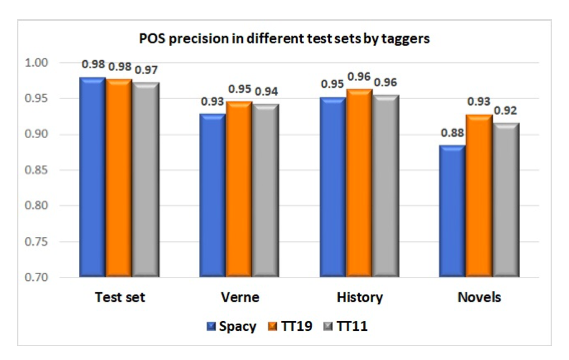
\includegraphics[width=.7\textwidth]{images/pos_tagger.png}
\caption{Preciznost alata za određivanje vrsta reči na različitim skupovima podataka}
\label{img:pos_tagger}
\end{figure}

\section{Lematizacija}

Proces lematizacije jeste onaj u kome se za svaku reč nalazi njena kanonska forma, tačnije lema. U srpskom jeziku, za imenice lema je nominativ jednine,  za glagole infinitiv, a za prideve nominativ jednine muškog roda. Takođe, proces lematizacije uključuje vraćanje rodne varijacije reči na njen pređašnji oblik.

Postoje dve metode za rešavanje problema lematizacije.  Prvi, da se prema obliku reči otklanja sufiks i nalazi njena lema. Ovaj oblik rešavanja ne daje tako dobre rezultate.  Drugi pristup uključuje korišćenje skupa podataka koji za svaku reč, za svaku njenu moguću vrstu reči, ima određenu lemu. Postoji mogućnost i kombinovanja ova dva pristupa. 

Algoritam korišćen u ovom radu za dobijanje vrsta reči je koriščen i za dobijanje lema. Korišćen je rečnik koji sadrži sve dozvoljene parove vrsta reči i lema za određenu reč.

Ovaj algoritam nije pravi lematizator, već na najverovatniju vrstu reči za određenu reč pridruži lemu koja se nalazi u rečniku. Zbog ovakov pristupa, reči koje za istu vrstu reči imaju različite leme ne mogu da postoje u rečniku \cite{tagger}.

Na slici \ref{img:lemmatization} je prikazana preciznost 3 različita modela lematizatora trenirana na različitim skupovima podataka. Slika je preuzeta iz \cite{tagger}.

\begin{figure}[h!]
\centering
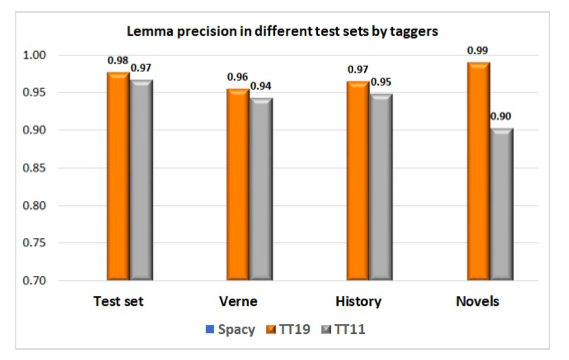
\includegraphics[width=.7\textwidth]{images/lemmatization.png}
\caption{Preciznost lematizatora na različitim skupovima podataka}
\label{img:lemmatization}
\end{figure}

\section{Skup podataka pre i nekon obrade}

Skup podataka koji će biti korišćen za eksperimente u ovom radu sadrži sakupljene podatke na već opisan način, koji su zatim obrađeni pomenutim tehnikama. Intervjui sa pacijentima obolelim od demencije Alchajmerovog tipa ima 22, koje nazivamo "pozitivni" i nalaze se u fascikli "P". Intervjui sa starijim licima koji nemaju utvrđenu demenciju Alchajmerovog tipa ima 57 i oni se nalaze u fascikli "N", a nazivamo ih "negativni". Nakon procesa određivanja vrste reci i leme za svaku reč intervjua, za svaki transkript je kreiran novi dokument koji u sebi sadrzi potrebne informacije. Ako se u transkriptu nalazi rečenica:
\newline
\newline
\noindent\fbox{
    \parbox{\textwidth}{
      Ja sam Bojana.  
    }
}
\newline
\newline
Onda će se u odgovarajućoj datoteci naći i sledeći redovi, gde u svakom prva reč označava izvorni oblik reči, druga vrstu, a treća lemu.
\newline
\newline
\noindent\fbox{
    \parbox{\textwidth}{
      Ja	ADV	Ja\newline
	sam	AUX	jesam\newline
	Bojana	PROPN	Bojana\newline
	.	PUNCT	.
    }
}
\newline
\newline

\chapter{Problem klasifikacije}

Pojam mašinskog učenja se vezuje za programe koji na osnovu podataka ”uče” kako da se ponašaju i zaključuju na prethodno nepoznatim podacima. Osnovna podela metoda mašinskog učenja je na nadgledano (eng. supervized) i nenadgledano (eng. unsupervized) učenje i učenje potkrepljivanjem TODO: mladen cite. Katarestika nadgledanog učenja je da se svaka instanca sastoji iz podatka od kog se uči i iz onoga što je potrebno naučiti. U slučaju klasifikacije, ono što se uči je sama klasa ili skup klasa koje se pridružuju podatku. Ova metoda rešava mnoge probleme, kao što je problem prepoznavanja lica, utvrđivanje prisustva bolesti i slično. Nenadgledano učenje se razlikuje po tome što instanca ne sadrži ono što je potrebno naučiti. Ove metode su fokusirane na nalaženje strukture u podacima, kao što je rešavanje problema klasterovanja. Učenje potkrepljivanjem se koristi gde je neophodno preduzeti niz akcija na osnovu stanja okruženja. Primer za ovu vrstu metoda je problem autonomne vožnje TODO: mladen cite.

Problem klasifikacije je jednostavan, od N klasa treba odrediti ispravnu za svaku instancu. Ulazni skup podataka koji se klasifikuje se sastoji od instanci. Klasifikacija spada u nadgledano učenje (eng. supervized), zato što su podaci koji se korste labelirani, uz sam podatak postoji i ranije određena klasa. Podaci se dele na dva skupa, za trening i test. Skup za trening služi da se nauče pravilnosti i izvedu zaključci, a skup za test služi za evaluaciju klasifikatora. Svi podaci prolaze korak pretprocesiranja koji uključuje obradu podataka kako bi ovaj proces bio uspešniji. Kreira se klasifikator, tačnije klasifikacioni model koji za zadatak ima da da preslika skup atributa instance x u neku od predefinisanih klasa y. Ulaz predstavlja skup atributa (eng. features) dok izlaz je najčešće jedna promenljiva koju nazivamo ciljnom promenljivom (eng. target variable). Ulaz se označava sa x, a izlaz sa y i obe promenljive su u vektorskom obliku.

Vrste klasifikacija se mogu podeliti po broju klasa, po tome da li može instanci biti dodeljeno više klasa ili samo jedna kao i po tipu klasifikacije.

Po broju klasa, podela je sledeća:

\begin{enumerate}
\item Binarna (eng. binary): postoje dve klase između kojih se bira i često odgovara na pitanje da li je nešto deo nekog skupa ili ne. Primer je detektcija nepoželjnih poruka ili pristustvo neke bolesti kod ispitanika.
\item Višeklasna (eng. multi-class): postoji više od dve klase između kojih se bira. Primer je prepoznavanje lica, klasifikacija vrste biljaka i slično. 
\end{enumerate}

Po tome da li može biti dodeljena samo jedna klasa ili više, podela je sledeća:

\begin{enumerate}
\item Jednoznačna (eng. single-label) - Jednoj instanci može biti dodeljena tačno jedna klasa
\item Višeznačna (eng.  multi-label) - Jednoj instanci se može pridružiti nula ili više klasa. Primer je kada na slici treba da se detektuju objekti, pa se očekuje prisutnost više objekata.
\end{enumerate}

Po tipu klasifikacije, razlikujemo sledeće:

\begin{enumerate}
\item Čvrsta (eng. hard) - Donosi se odluka da li instanca pripada klasi ili ne. 
\item Meka (eng. soft) - Instanci se pridružuje vrednost između 0 i 1 i time se određuje pripadnost klasi. TODO:cite
\end{enumerate}

\begin{figure}[h!]
\centering
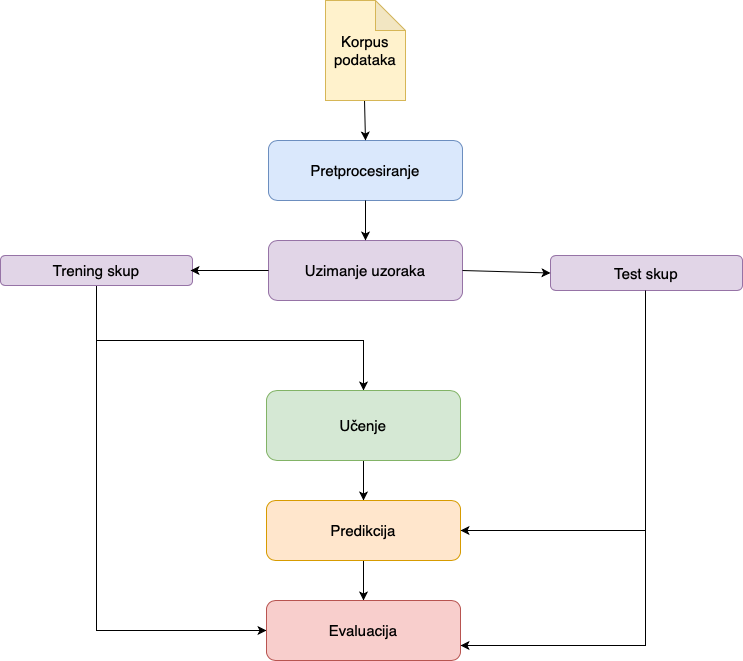
\includegraphics[width=.7\textwidth]{images/workflow.png}
\caption{Proces klasifikacije}
\label{img:workflow}
\end{figure}

Na slici \ref{img:workflow} je prikazan tok rada klasifikacije. Prvi korak je skupljanje podataka i njihova obrada, zatim deljenje na test i trening skup. Na ovakvim skupovima se radi pretprocesiranje i obrada podataka. Trening skup zatim služi za treniranje klasifikatora. Uz pomoć tog istreniranog klasifikatora se radi predikcija na skupu za testiranje. Nakon toga, sledi neophodan korak evaluacije modela u koji ulazi procena performansi. Bitno je naglasiti da se većina ovih koraka ne izvodi jednom i svi koraci od učenja do evaluacije se izvode veliki broj puta kako bi se dobila najbolja moguća tačnost. Klasifikator se mora prilagoditi podacima, kako deo izbora algoritma, tako i podešavanje njegovih parametara.

U narednim sekcijama će bliže biti objašnjeni ovi koraci.  

\section{Podela korpusa}

Ulazni skup, korpus, se deli na dve grupe, za trening i za test. Skup za treniranje se naziva trening skup i služi za kreiranje klasifikatora. Skup za testiranje se naziva testni skup i služi za evaluaciju klasifikatora. U većini slučajeva testni skup predstavlja manji deo korpusa od trening skupa. Korak deljenja korpusa na trening i testni skup se naziva stratifikacija \cite{MarijaMR}. Neophodno je da skupovi budu ravnopravno raspodeljeni. Oba skupa treba da reprezentuju ceo uzorak koji se razmatra. U svakom skupu treba da se nađe određeni procenat obe klase koje razmatramo. Korpus delimo na ove dve grupe na osnovu jedne karakteristike koja je izabrana, a u slučaju klasifikacije je najčešće to baš ona karakteristika koja određuje kojoj klasi uzorak pripada. U slučaju klasifikacije obolelih od Alchajmera, karakteristika koju biramo je pripadnost pozitivnom i negativnom korpusu, tačnije da li je osoba obolela od Alchajmera ili ne.  

U slučaju podataka koji se koriste za eksperimente u ovom radu, skupovi pozitivnih i negativnih su oba podeljena na tri podskupa, pa tako skup za treniranje se sastoji iz dva podskupa pozitivnih i 2 podskupa negativnih, a skup za testiranje iz trećeg podskupa pozitivnih i trećeg podskupa negativnih. Ovakva podela je napravljena zbog malog broja instanci u korpusu koje su prikupljene.

\section{Pretprocesiranje}
 
Pretprocesiranje je korak koji nije obavezan, ali može značajno poboljšati performanse klasifikatora. Pretprocesiranje se koristi za prečišćavanje teksta, uklanjanje reči koje nisu bitne za klasifikaciju i za uniformisanje reči. Metode pretprocesiranja teksta su različite u zavisnosti od podataka koji se koriste. Nakon prikupljanja podataka, korpus predstavljaju sirovi podaci. Svaki tekst se deli na reči i zatim se pirstupa nekim od tehnika pretprocesiranja:

\begin{enumerate}
\item Određivanje vrsta reči
\item Stemovanje
\item Lematizacija
\item Uklanjanje razmaka
\item Uklanjanje stop reči
\item Uklanjanje znakova interpunkcije
\item Prevođenje velikih slova u mala
\item Normalizacija teksta
\end{enumerate}

\textbf{Određivanje vrsta reči} je postupak gde se svakoj reči u rečenici pridružuje njena vrsta. Zadatak je takav da dodeljujemo svakoj reči $x_i$ u ulaznoj sekvenci reči labelu $y_i$,  tako da izlazna sekvenca Y ima istu dužinu kao ulazna sekvenca X \cite{postagging}. Reči imaju više mogućih vrsta reči i zadatak ovog procesa je da se pronađe ispravna vrsta reči za svaku pojedinu situaciju. U prethodnom poglavlju je bliže objašnjen algoritam kako program korišćen funkcioniše.

\textbf{Stemovanje} je proces uklanjanja sufiksa ili prefiksa reči. Ovim postupkom se nalazi koren reči. Problemi koji se mogu susresti su prekomerno ili premalo stemovanje, kada se uklanja veći deo reči nego što treba, ili manji.

\textbf{Lematizacija} je sličan proces, ali se reč vraća na njen oblik iz rečnika, tačnije lemu. U srpskom jeziku, za imenice lema je nominativ jednine,  za glagole infinitiv, a za prideve nominativ jednine muškog roda. U okviru prethodnog poglavlja je detaljnije objašnjen proces lamatizaije kao i objašnjen algoritam korišćen u ovom radu. Stemovanjem i lematizacijom se reči koje su zapisane u različitim oblicima, a imaju isto značenje, prevode u isti oblik.

\textbf{Uklanjanje razmaka i znakova interpunkcije} je jednostavan zadatak, a bitno je ukloniti ih pošto nemaju značaj u razumevanju teksta.
 
\textbf{Prevođenje velikih slova u mala} je takođe sa strane implementacije jednostavan zadatak, a često se previdi. Ovaj korak pomaže u tome da se unifikuju reči i da nije bitno gde u rečenici je izgovorena reč i da li je napravljena greška u kucanju.

Korak \textbf{uklanjanja stop reči} se sastoji iz uklanjanja reči koje se često pojavljuju u jeziku. Neke od stop reči u srpskom jeziku su "bi", "da", "li", "čega", "će", "ću", "ga", "ja" i slične. Stop reči nisu relevantne za klasifikaciju, pa se uklanjaju da ne bi skidale fokus sa onih koje su bitne.

Korak \textbf{normalizacije} teksta se izvodi tako što se svaka reči koja se nalazi u nestandardnom obliku prevodi u kanonsi oblik. Ovaj korak je bitan ukoliko se u tekstu nalaze žargonski izrazi, skraćenice i slično. TODO: tag Maja.

U okviru ovog rada su koraci određivanja vrsta reči i lematizacija odrađeni pre deljenja teksta na skupove za testiranje i treniranje. U okviru metoda mašinskog učenja koje će biti prikazane u nastavku su korišćeni koraci uklanjanja razmaka, stop reči i razmaka, kao i prevođenje velikih slova u mala.


\section{Vektorska reprezentacija teksta}

Korpus podataka se sastoji od tekstova i klase.  Tekst u svojoj klasičnoj formi nije pogodan ulaz za algoritme mašinskog učenja.  Pošto se na ulazu očekuju numeričke vrednosti,  potreban je mehanizam koji će preslikati tekst u brojčani format na neki logičan način.  Upravo taj korak se naziva ugrađivanje reči(eng.  word embedding) TODO:  Maja cite 
Metode koje ćemo razmotriti u okviru ovog rada:

\begin{enumerate}
\item Vreća reči
\item N-grami 
\item FA mera
\item FA-IFD mera
\end{enumerate}

\subsection{Vreća reči}
Vreća reči (eng. bag-of-words) je jednostavna tehnika reprezentacije teksta i način na koji se izdvajaju svojstva teksta.  Ovom reprezentacijom se prikazuje koliko puta se neka reč nalazi u dokumentu.  Redosled reči u rečenici nije bitan,  pa je odatle i dobila svoje ime ”vreća”.  Ova reprezentacija takođe omogućava da ulaz u algoritam mašinskog učenja bude vektor fiksne dužine,  što daje strukturu ulaza i to je pogodno za ovakve algoritme.  Vreća reči i pored toga što se kontekst i semantika zanemaruju,  često daje dobre rezultate.  
Pretprocesiranje dokumenata pre prevođenja u ovu reprezentaciju je bitno zato što su skupovi nad kojima se uči tipično jako veliki, a ovaj korak će smanjiti dimenziju rečnika koji se kreira, pa i reprezentacije svakog dokumenta.  
U okviru programskog jezika Python postoji biblioteka Sklearn koja u sebi sadrži CountVectorizer objekat koji se može korisitit za implementaciju i koji je korišćen u za eksperimente u ovom radu. 
Na primeru ćemo pokazati kako se kreira vreća reči:

\subsubsection{Predstavljanje korpusa}
Korpus nam predstavljaju 3 dokumenta:
\newline
\newline
\noindent\fbox{
    \parbox{\textwidth}{
    	1. Zorica voli da vežba u teretani. \newline
	2. Jovana voli da vežba jogu uveče.\newline
	3. Marko ne voli da vežba, ali voli da šeta u šumi.
    }
}
\newline
\newline
\subsubsection{Pretprocesiranje i deljenje na reči}
Kao korak pretprocesiranja,  uklonjeni će biti svi znakovi interpunkcije,  svi nepotrebni razmaci i sva slova će biti prevedena u mala,  uklonjene su stop reči i izvršena je lematizacija. U sledećem koraku će svaki dokument biti podeljen na reči.  Dokumenti sada izgledaju ovako:
\newline
\newline
\noindent\fbox{
    \parbox{\textwidth}{
    	1. "zorica", "voli", "vežba", "teretana" \newline
	2. "jovana", "voli", "vežba","joga",  "uveče"\newline
	3. "marko", "ne", "voli", "vežba", "voli", "šeta", "šuma"
    }
}
\newline
\subsubsection{Rečnik}
Zatim kreiramo rečnik od svih reči koje se nalaze u svim dokumentima korpusa koji su prikazani u prošlom koraku.  Reči su sortirane. 
\newline
\newline
\noindent\fbox{
    \parbox{\textwidth}{
    	["joga", "jovana",  "marko", "ne", "šeta", "šuma", "uveče", "vežba", "voli", "teretana", "zorica" ]
    }
}
\newline
\subsubsection{Predstavljanje dokumenata vrećom reči}
U sledećem koraku transformišemo dokumente na osnovu pojavljivanja reči iz rečnika. 
\newline
\newline
\noindent\fbox{
    \parbox{\textwidth}{
    	1.  [0, 0, 0, 0, 0, 0, 0, 1, 1, 1, 1] \newline
	2.  [1, 1, 0, 0, 0, 0, 1, 1, 1, 0, 0] \newline
	3. [0, 0, 1, 1, 1, 1, 0, 1, 2, 0, 0]
    }
}
\newline
Trening skup se iz početnog koji sadrži dokumente transformiše u niz od n elemenata, gde je n broj dokumenata u korpusu.  Svaki element je jedan niz koji ima m elemenata, gde je m dužina rečnika.  Testni skup se na identičan način preslikava iz dokumenata u niz vekora.  
Vrećom reči se je reprezentovan samo broj pojavljivanja reči u dokumentu.  Ako se neka reč pojavljuje mnogo puta, to ne mora nužno značiti da je ona bitna.  Možda se samo često pojavljuje u tom skupu podataka ili je reč koja se često izgovara.

\subsection{N-grami}

\newtheorem{mydef}{Definicija}
\begin{mydef}
Za datu sekvencu tokena S = \normalfont($s_1$,$s_2$,...,$s_{N+(n-1)}$\normalfont) , gde su N i n pozitivne celobrojne vrednosti,  n-gram sekvence S je podsekvenca uzastopnih tokena dužine n.  i-ti n-gram sekvence S je sekvenca ($s_i$, $s_{i+1}$, ..., $s_{i+n-1}$) TODO
\end{mydef}

N-gram predstavlja n sekvencijalnih elemenata.  N-grami se mogu definisati na nivou reči, karaktera i bajta.  N-grami na nivou karaktera i bajta su kod jezika koji se pišu latiničnom azbukom slučni,  zato što jedan karakter predstavlja jedan znak, ali to nije slučaj kada je u pitanju na primer azijski jezici.  N-gramski model pokušava da nauči šablon sekvenci.  Ovom modelu su bitne i relacije između elementa, koji se pojavljuje blizu kog.  N-gramski model se čuva donekle poredak reči.  Razmatra se mogućnost da se određeni element e nađe posle određene sekvence elemenata s. 
Korišćenje n-grama se u okviru procesa obrade prirodnih jezika pokazalo kao efikasno.  Ova tehnika se koristi vrlo često u predviđanju reči koje se nadovezuju na datu rečenicu, ispravljanju grešaka u pisanju, generisanju teksta i slično.  
N-grami su relativno neosetljivi na pravopisne greške i jednostavni za implementaciju, pa se pre korišćenja ovog modela ne radi korak pretprocesiranja teksta, već samo izbacivanje znakova interpunkcije.  
Kod n-gramskih modela se n broj bira prema prirodi problema i podataka,  ali se najčešće koriste brojevi do n=5.  Kada je n=1 to su unigrami, kada je n=2 to su bigrami,  a kada je n=3 to su trigrami i tako dalje.  Nekada se koriste i njihove kombinacije. 
U nastavku će biti pokazani primeri n-grama reči.

\subsubsection{Predstavljanje korpusa}
Korpus nam predstavljaju 3 dokumenta:
\newline
\newline
\noindent\fbox{
    \parbox{\textwidth}{
    	1. Zorica voli da vežba u teretani. \newline
	2. Jovana voli da vežba jogu uveče.\newline
	3. Marko ne voli da vežba, ali voli da šeta u šumi.
    }
}
\newline
\newline

\subsubsection{Unigrami}
Unigrami su n-grami gde je n=1. Ovaj model liči na vreću reči, sa razlikom da se kod n-grama ne vrši pretprocesiranje,  pa će biti više izdvojenih reči.  Kod unigrama nema oslanjanja na prethodnu sekvencu s. 
Unigrami u primeru su sledeći:
\newline
\newline
\noindent\fbox{
    \parbox{\textwidth}{
    	1. "zorica","voli", "da",  "vežba", " u", "teretani" \newline
	2. "jovana", "voli", "da", "vežba", "jogu",  "uveče"\newline
	3. "marko", "ne", "voli", "da", "vežba","ali", "voli", "da", "šeta", "u", "šumi"
    }
}
\newline
\newline

\subsubsection{Bigrami}

Bigrami su n-grami gde je n=2.  Sekvenca elemenata s koja se nalazi pre elementa koji se trenutno gleda je samo jedna reč.  Bigrami su u stanju da uzmu u obzir i negaciju, zato sto gledaju dve reči zajedno, pa ovakvi modeli mogu dati i bolje rezultate.   
Bigrami u primeru su sledeći: TODO: cite Maja
\newline
\newline
\noindent\fbox{
    \parbox{\textwidth}{
    	1.  ("zorica","voli"),("voli","da"), ("da", "vežba"), ("vežba",  "u"), ("u", "teretani")  \newline
	2.  ("jovana", "voli"),  ("voli","da" ), ("da", "vežba"), ("vežba", "jogu"), ("jogu","uveče" ) \newline
	3.  ("marko", "ne"), ("ne", "voli"), ("voli", "da"), ("da", "vežba"), ("vežba","ali" ), ("ali", "voli" ),("voli","da" ), ("da", "šeta"), ("šeta", "u"), 		("u","šumi")
    }
}
\newline
\newline
\subsubsection{Trigrami}
Trigrami su n-grami gde je n=3. Trigrami u primeru su sledeći:
\newline
\newline
\noindent\fbox{
    \parbox{\textwidth}{
    	1.  ("zorica","voli", "da"),("voli","da", "vežba"), ("da", "vežba", "u"), ("vežba","u","teretani")\newline
	2.  ("jovana", "voli", "da"),  ("voli","da","vežba" ), ("da", "vežba", "jogu"), ("vežba", "jogu", "uveče") \newline
	3.  ("marko", "ne", "voli"), ("ne", "voli", "da"), ("voli", "da", "vežba"), ("da", "vežba", "ali"), ("vežba","ali", "voli"), ("ali", "voli","da"),			("voli","da","šeta"), ("da", "šeta","u"), ("šeta", "u", "šumi")
    }
}
\newline
\newline

Na prethodnom primeru je prikazan način na koji se grade n-grami reči. Na isti način se grade i n-grami karaktera i bajtova.  
\subsection{Frekvencija atributa - FA}

Frekvencija atributa (eng. term frequency) se označava sa FA (eng. TF) meri učestalost pojavljivanja reču i dokumentima.  Učestalije reči imaju veću važnost od onih manje učestalih.  FA mera pokazuje koliko se često se određeni atribut w nalazi u dokumentu. 
 Da bi se izbegao slučaj da neka reč ima veću frekvenciju pojavljivanja, a samim tim i veću bitnost, samim tim što je dokument veći, uvodi se normalizacija tako što se broj pojavljivanja reči u tekstu podeli sa ukupnim brojem reči u tekstu.  Ovaj model daje bolje rezultate ukoliko je u okviru pretprocesiranja odrađeno izbacivanje stop reči, kao i uklanjanje znakova interpunkcije i lematizacija.  Frekvencija atributa se može kreirati nad vrećom reči kao i nad n-gramima.  TODO maja cite
Računa po formuli za reč w i dokument d:

\begin{equation}
	FA(w,d) = \frac{\text{broj pojavljivanja reči w u dokumentu d}}{\text{broj svih reči u dokumentu d}}
\end{equation}

\subsection{Inverzna frekvencija dokumenta - IFD}

Frekvencija dokumenta (eng.  document frequency) se označava kao FD (eng.  DF) se definiše kao broj dokumenata u kojima se pojavljuje atrubut w.  Uvodimo oznaku:
\begin{equation}
	FD(w) = \text{broj svih dokumenata u kojima se pojavljuje reč w}
\end{equation}

Inverzna funkcija frekvencije dokumenta (eng.  inverse document frequency) tog atributa se se predstavlja kao broj dokumenata u korpusu u onosu na broj dokumenata u kojima se pojavljuje atribut w i računa se po formuli:

\begin{equation}
	IFD(w) = \frac{\text{broj svih dokumenata u korpusu}}{\text{broj svih dokumenata u kojima se pojavljuje reč w}}
\end{equation}

Kada je korpus veliki,  vrednost inverzne fkrekvencije dokumenata može biti ogroman broj, pa se dodaje logaritamska funkcija.  Da bi se izbeglo deljenje sa nulom, ako se reč ne pojavljuje u dokumentu,  dodaje se vrednost 1, pa formula izgleda ovako:

\begin{equation}
	IFD(w) = log\left(\frac{\text{broj svih dokumenata u korpusu}}{FD(w) + 1}\right)
\end{equation}

\subsection{FA-IFD metrika}

Prethodne mere se mogu kombinovati u jednu koju nazivamo FA-IFD (eng.  TD-IDF), tako da se nađu atributi koji imaju veliku frekvenicu atributa,  a malu frekvenciju dokumenata, pošto je cilj da se da na važnosti atributima koji su frekventni u pojedinačnim dokumentima, a da se retko pojavljuju u ostalim dokumentimaTODO: add JElena.  Ova mera je zapravo proizvod prethodnih mera i formula izgleda ovako:

\begin{equation}
	FA-IFD(w, d) = FA(w,d) * IFD(w)
\end{equation}

Frekvencija atributa se može kreirati nad vrećom reči kao i nad n-gramima.  U implementaciji ovog rada će biti prikazane obe opcije.

\section{Kreiranje i treniranje modela}

Za treniranje modela neophodno je odrediti algoritam koji će se koristiti za kreiranje klasifikatora. U zavisnosti od prirode problema, vrste i količine podataka, ali i vrste podataka se bira algoritam koji će dati najbolje performanse. Klasifikator se trenira samo nad podacima za trening, što je prikazano na slici 3.1 TODO:Referenca na sliku. U ovom koraku se na podacima koji su raspoloživi u skupu za treniranje model ”uči” i nalazi pravilnosti. U koraku predikcije predviđa na testnom skupu koji nije korišćen u koraku treniranja.

U okviru ovog rada će biti prikazan klasifikator razvijen na lingvističkim metodama u četvrtom poglavlju, Naivni Bajesov klasifikator koji će biti prikazan u petom poglavlju i klasifikator baziran na metodi podržavajućih vektora u šestom poglavlju.

\section{Evaluacija modela}

Poslednji korak je određivanje koliko je model koji je napravljen zapravo dobro isteniran. Poređenjem predviđene klase i one stvarne dolazimo do zaključaka. Jedan od problema koji se može javiti je problem previše prilagođenog modela, a javlja se ukoliko se klasifikator previše prilagodi podacima za treniranje.  Ovaj problem se može detektovati tako što su rezultati na skupu za treniranje dobri, dok su performanse na test skupu loše.  Najčešće se javlja kada se šum u ulaznim podacima predstavi kao bitan element.  TODO: jelena

Instance koje se nalaze u test skupu nisu korišćene za kreiranje modela i za svaku od njih klasifikator predviđa klasu. Nakon ovog koraka se uz svaki dokument iz test skupa nalaze dve klase, ona koju znamo da je tačna i ona dodeljena klasifikatorom. Svaki dokument može biti ispravno i neispravno klasifikovan i prema tome može biti u skupu:

\begin{enumerate}
\item Stvarno pozitivni SP (eng. True Positives, TP)
\item Lažno pozitivni LP (eng. False Positives, FP)
\item Stvarno negativni SN (eng. True Negative, TP)
\item Lažno negativni LN (eng. False Negative, FN)
\end{enumerate}
\noindent
gde je stvarno pozitivni broj instanci koje su zaista pozitivne i koje je klasifikator označio kao pozitivne. Lažno pozitivni je broj instanci koje su negativne, a koje je klasifikator označio kao pozitivne. Stvarno negativni je broj instanci koje su negativne, a koje je klasifikator označio kao negativne. Lažno negativni je broj instanci koje su pozitivne, a koje je klasifikator označio kao negativne. Njihov zbir treba da bude jednak broju instanci u testnom skupu.

Ova četiri podatka definišu matricu konfuzije (eng. confusion matrix). Matrica konfuzije je NxN matrica koja se koristi za evaluaciju klasifikacionog modela, gde je N broj klasifikacionih klasa. U slučaju višeklasne klasifikacije element matrice C\textsubscript{ij} predstavlja broj elemenata koji pripadaju klasi i, a klasifikovani su u klasu j \cite{MarijaMR}. Model je bolji što je više elemenata van dijagonale u matrici jednako nula. Matrica konfuzije za binarnu klasifikaciju je prikazana na slici \ref{img:confusionMatrix}.

\begin{figure}[h!]
\centering
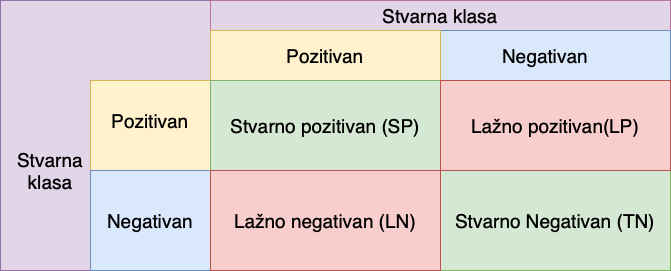
\includegraphics[width=.7\textwidth]{images/confusionMatrix.png}
\caption{Matrica konfuzije}
\label{img:confusionMatrix}
\end{figure}

Ove podatke koristimo za procenu koliko je model dobro istreniran pomoću određenih mera, a neke od njih su sledeće:

\begin{enumerate}
\item Tačnost klasifikacije
\item Preciznost klasifikacije
\item Odziv klasifikacije
\item F-mera
\end{enumerate}

Tačnost klasifikacije (eng. accuracy) prikazuje odnos tačno klasifikovanih instanci i svih klasifikovanih instanci i računa se po formuli:

\begin{equation}
	acc = \frac{SP+SN}{SP+SN+LP+LN}
\end{equation}

Preciznost klasifikacije (eng. precision) prikazuje odnos pozitivnih instanci koje su tako klasifikovane i svih instanci koje su klasifikovane pozitivno i računa se po formuli:

\begin{equation}
	P = \frac{SP}{SP+LP}
\end{equation}

Ova mera pokazuje koliko je instanci pogrešno klasifikovano kao pozitivno. Ako model nema lažnih pozitiva (LP), onda će vrednost preciznosti biti 1, tačnije 100\%. Što više lažnih pozitiva ima, to će preciznost biti lošija. Vrednosti preciznosti se kreću između 0 i 1.

Odziv klasifikacije (eng. recall) je mera koja prikazuje odnos pozitivnih instanci koje su tako klasifikovane i zbira pozitivnih instanci koje su tako klasifikovane i pozitivnih instanci koje su klasifikovane kao negativne. Ova mera se fokusira na broj pozitivnih instanci koje su pogrešno klasifikovane. Ako su sve pozitivne instance upravo tako klasifikovane, onda će vrednost odziva biti 1, tačnije 100\%. Računa se po formuli:

\begin{equation}
	R = \frac{SP}{SP+LN}
\end{equation}

Preciznost je bitna mera kada nam je bitnija mera lažno pozitivnih od lažno negativnih. Preciznost je bitna mera u sistemima gde je bitno da se ne dobije negativan rezultat, dok je odziv bitna mera u sistemina gde je problem ako pozitivan slučaj prođe nezapaženo.

F-mera predstavlja harmonijsku sredinu preciznosti i odziva i razmatra i lažno pozitivne i lažno negativne. Računa se po sledećoj formuli:

\begin{equation}
	F = \frac{2}{\frac{1}{P} + \frac{1}{R}} = \frac{2 * P * R }{P + R}
\end{equation}

Unakrsna validacija (eng.  k-cross validation) se takođe može uraditi u cilju evaluacije modela. Ova metoda podrazumeva višestruko izvođenje koraka treniranja i evaluacije nad različitim skupovima, da bi se na kraju našla srednja vrednost neke od mera kao što je tačnost modela. Korpus podataka se deli na ranije određen K broj skupova, gde se proces treniranja izvodi na K-1 skupu, a preostali skup se koristi za testiranje. U svakom koraku se menjaju skupovi za trening i test, tako da testni skup bude svaki put različit i ovaj postupak se ponavlja K puta. Parametar K se bira prema korpusu podataka. U slučaju implementacije prikazane u ovom radu, izabran je K = 3. Unakrsna validacija za K = prikazana na slici \ref{img:K_cross_validation}, gde svaki red predstavlja jednu iteraciju treniranja, testiranja i evaluacije, ljubičast kvadrat prikazuje skup za testiranje, a beli kvadrati skupove za treniranje.

\begin{figure}[h!]
\centering
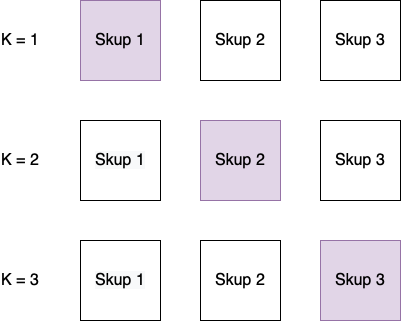
\includegraphics[width=.7\textwidth]{images/K_cross_validation.png}
\caption{Unakrsna validacija}
\label{img:K_cross_validation}
\end{figure}


\chapter{Rešavanje problema metodama lingvističke analize}

Lingvistička analiza predstavlja pokušaj da računar zaključuje na osnovu značenja taksta i tada kažemo da se sprovodi obrada prirodnog jezika (eng. Natrual Language Processing).  Da bi računar razumeo pisani tekst,  prvo je neophodno podeliti ga na rečenice.  Mnogi lingvistički alati se baziraju na analizi jedne po jedne rečenice.  Zatim se izvodi proces tokenizacije,  deljenja rečenice na pojedinačne reči.  Nakon toga je se izvodi korak lematizacije,  prevođenja svake reči u njen osnovi oblik, tačnije lemu.  U nekim slučajevima,  ovaj korak obukvata i čišćenje, tačnije ispravljanje pogrešno napisanih reči.  Poslednji korak je dodeljivanje vrsta reči svakoj od njih (eng. Part of speech tagging). 
Pacijenti oboleli od Alchajmerove bolesti kao jedan od simptoma imaju gubitak sposobnosti funkcionalne komunikacije i probleme u lingvističkim veštinama.  Procenjivanje afazije kod pacijenata obolelih od demencije Alzhajmerovog tipa je vrlo zahtevan zadatak.  Koristeći različite metrike nad vrstama reči koje su dobijene iz spontanog govora obolelih,  pokušavamo da pronađemo pravilnost i da tako dođemo do zaključaka i mogućnosti klasifikacije na obolele i zdrave pojedince.  
U mnogim naučnim radovima koji se bave temom Alchajmerove bolesti se predstavljaju upravo lingvističke mere kao način razlikovanja obolelih od zdravih pojedinaca i metod za uočavanje pravilosti u njihovom govoru. Potrebno je naći pravilnost u načinu na koji pojedinac govori i koristi svoj vokabular, koliko često izgovara neke vrste reči,  koliko su dugačke rečenice.  Neki od primera korišćenja ovih mera se mogu naći u radovima , \cite{automaticdetandrat}, \cite{Evaloftechfolexicalperformance} i \cite{linguisticfeatures}.

\section{Lingvističke mere}

Korišćeno je ukupno šesnaest mera u okviru ovog rada.  Mere bazinare na vrstama reči uključuju frekvenciju pojavljivanja određene vrste reči u tekstu, kao i tu vrednost normalizovanu ukupnim brojem reči u tekstu. Takođe,  koriste se tri mere: Odnos tipa tokena (eng.  Type Token Ratio),  Brunetova statistika (eng. Brunet's Statistic) i Honoreva statistika (eng.  Honore's Statistic) koje počivaju na bogatstvu vokabulara. 
Za svaki tekst se izračunava dužina teksta (N) kao broj izgovorenih reči i prosečna dužina izgovorenih reči.  Vokabular(V) je mera koja pokazuje koliko različitih reči se pojavljuje u tekstu koji se obrađuje.  Vokabular reči izgovorenih jednom (V\textsubscript{1}) se izračunava tako što se od reči koje se nalaze u vokabularu broje samo one koje su izgovorene jednom.  Ove mere se koriste kako samostalno, tako i za izračunavanje mera koje počivaju na bogatstvu vokabulara. 
\break

\section{Mere bazirane na vrstama reči}

Mera pojavljivanja pojedinačne vrste reči u tekstu se izračunava tako što se broji svako pojavljivanje te vrste reči.  Pored toga,  izračunavamo i frekvencije pojavljivanja različitih vrsta reči normalizovane ukupnim brojem reči u tekstu.  U okviru ovog rada, razmatrane su mere vezane količinu imenica,  glagola,  prideva, priloga i zamenica kao i njihove normalizovane vrednosti.  Od koristi mogu biti i odnosi između ovih vrednosti, pa se tako izračunavaju i odnos između količine pojavljivanja imenica i glagola,  zamenica i imenica i zamenica i glagola.  (TODO: Proveriti i ostale, sa pridevima npr.) Ove mere su izabrane heuristički i predstavljaju leksičku raspodeljenost izgovorenih reči.  
Količina imenica pokazuje sposobnost ispitanika da koristi imenice i ona bi mogla biti osetljiva na probleme sa pronalaženjem reči od čega pate osobe koje imaju Alchajmerovu bolest. Količina zamenica je u konstrastu sa količinom imenica i koristi se kao merilo indirektnog referenciranja.  Količina prideva prikazuje kvalitet govora obolele osobe, tačnije mogućnost za opisivanjem. Količina glagola se često koristi kao lingvistička mera i meri tečnost govora. \cite{Evaloftechfolexicalperformance}.  Ove mere su korišćene u mnogim prethodnim istraživanjima kao što su \cite{automaticdetandrat}, \cite{Evaloftechfolexicalperformance} i \cite{linguisticfeatures}. 

\section{Mere bazirane na bogatstvu vokabulara}
 
Tri mere koje se zasnivaju na bogatstvu vokabulara su: Odnos tipa tokena (eng. Type Token Ratio),  Brunetova statistika (Brunet's Statistic) i Honoreva statistika (Honore's Statistic).  Za njihovo izračunavanje neophodno je prvo izračunati dužinu teksta, bogatstvo vokabulara i bogatstvo vokabulara za reči izrečene jednom.  Dužina teksta se meri kao broj reči koje se pojavljuju u tekstu i označava se sa N.  Mera bogatstva vokabulara se izračunava tako što se broji koliko različitih reči se pojavljuje u tekstu i označava se sa V. Mera bogatstva vokabulara za reči izgovorene jednom se izračunava tako što se broje reči u tekstu koje se pojavljuju samo jednom.  Ova mera se označava sa V\textsubscript{1} .  

\subsection{Odnos tipa tokena}

Odnos tipa tokena (eng. Type Token Ratio) se računa po formuli:

\begin{equation}
	TTR = \frac{V}{N}
\end{equation}

{\setlength{\parindent}{0cm}
gde je N dužina teksta, a V mera bogatstva vokabulara i predstavlja odnos ove dve vrednosti. Ova mera je osetljiva na dužinu teksta.  Veće vrednosti odnosa tipa tokena se povezuju sa bogatijim vokabularom. 
}
\subsection{Brunetov Indeks}

Brunetov indeks (eng. Brunet's Statistic) se računa po formuli:

\begin{equation}
	W = N^{V^-0.165}
\end{equation}
{\setlength{\parindent}{0cm}
gde je N dužina teksta, a V mera bogatstva vokabulara. Ova mera se takođe povezuje sa bogatijim vokabularom, ali nije osetljiva na dužinu teksta.  Tipične vrednosti su između 10 i 20.  Manje vrednosti se povezuju sa bogatijim govorom. 
}
\subsection{Honoreva Statistika}

Honoreva Statistika (eng. Honore's Statistic) se računa po formuli:

\begin{equation}
	R = \frac{100logN}{1 - \frac{V_1}{V}}
\end{equation}
{\setlength{\parindent}{0cm}
gde je N dužina teksta, a V mera bogatstva vokabulara, a V\textsubscript{1} bogatstvo vokabulara za reči izrečene jednom.  Veće vrednosti se povezuju sa bogatijim govorom.  
}
\section{Klasifikacija bazirana na lingvističkim merama}

Za izračunavanje mera pomenutih u prethodnim sekcijama,  koje nazivamo lingvističkim,  koriste se već obrađeni podaci u kojima je svakoj reči svakog teksta pridružena njena vrsta.  Izračunavanje mera koristeći tako pripremljene tekstove nije teško.  Mere izračunavamo za svaki tekst pojedinačno u korpusu koji sadrži kako pozitivno, tako i negativno klasifikovane tekstove.  Mere čuvamo u okviru datoteke koja nosi ime ispitanika sa ekstenzijom .txt. Ovakve mere možemo koristiti za upoređivanje i vizuelno prikazivanje na grafikonima. Da bismo procenili koliko je neka od metrika korisna u proceni da li je neko oboleo od Alchajmerove bolesti ili ne,  moramo na osnovu nje pokušati da klasifikujemo novi tekst kao pozitivan ili negativan.  Ova vrsta klasifikacije se naziva binarna klasifikacija. 

Korak treniranja modela u ovom slučaju je već odrađen, pošto već imamo sve metrike izračunate za trening skup. Vrednosti metrika iz trening skupa ćemo u koraku evaluacije porediti sa vrednostima metrika iz testnog skupa.

Korak evaluacije u ovom slučaju obuhvata procenu kvaliteta klasifikacije za svaku od metrika koje smo pomenuli u prethodnim sekcijama.  Vrednosti metrike za jedan tekst iz testnog skupa poredimo sa svim vrednostima metrika iz trening skupa i prema blizini odlučujemo kom od skupova tekst iz testnog skupa treba da pripadne po našem klasifikatoru. Zatim se klasa poredi sa stvarnom klasom koju tekst nosi. 

Ako pretpostavimo da trening i test skup sadrže sledeće dokumente:

\begin{equation}
	TRENING = {d\textsubscript{1}, d\textsubscript{2}, d\textsubscript{3},d \textsubscript{4}}
\end{equation}

\begin{equation}
	TEST = {d\textsubscript{5}}
\end{equation}
{\setlength{\parindent}{0cm}
gde dokumenti d\textsubscript{1}, i d\textsubscript{2} pripadaju skupu P,  a dokumenti d\textsubscript{3}, i d\textsubscript{4} skupu N, a d\textsubscript{5} pripada skupu P
}
i da radimo klasifikaciju po metrici X, onda sledi izračunavanje:

\begin{align}
	y\textsubscript{1} = \text{abs}(\text{X}(d\textsubscript{1}) - \text{X}(d\textsubscript{5})) \\
	y\textsubscript{2} = \text{abs}(\text{X}(d\textsubscript{2}) - \text{X}(d\textsubscript{5})) \\
	y\textsubscript{3} = \text{abs}(\text{X}(d\textsubscript{3}) - \text{X}(d\textsubscript{5})) \\
	y\textsubscript{4} = \text{abs}(\text{X}(d\textsubscript{4}) - \text{X}(d\textsubscript{5})) \\
	y\textsubscript{P} = y\textsubscript{1} + y\textsubscript{2} \\
	y\textsubscript{N} = y\textsubscript{3} + y\textsubscript{4}
\end{align}
gde (\text{X}(d\textsubscript{i}) predstavlja vrednost metrike X u dokumentu d\textsubscript{i}.
{\setlength{\parindent}{0cm}
Zatim se porede vrednosti y\textsubscript{P} i y\textsubscript{N}.  Koja vrednost je manja,  smatramo da dokument toj grupi pripada posto je ukupan zbir razlika vrednosti između dokumenta {d\textsubscript{5}} od dokumenta iz te grupe manji.  

Sledeći korak je evaluacija modela koja je bliže opisana u sekciji 3.5. Nakon što su dobijene vrednosti,  svaki dokument označavamo jednom od ovih oznaka:
}
\begin{enumerate}
\item Stvarno pozitivni SP (eng. True Positives, TP)
\item Lažno pozitivni LP (eng.  False Positives,  FP)
\item Stvarno negativni SN (eng.  True Negative, TP)
\item Lažno negativni LN (eng.  False Negative, FN)
\end{enumerate}
{\setlength{\parindent}{0cm}
gde je stvarno pozitivni broj instanci koje su zaista pozitivne i koje je klasifikator označio kao pozitivne.  Lažno pozitivni je broj instanci koje su negativne, a koje je klasifikator označio kao pozitivne.  Stvarno negativni je broj instanci koje su negativne,  a koje je klasifikator označio kao negativne.  Lažno negativni je broj instanci koje su pozitivne, a koje je klasifikator označio kao negativne.  Kada se ovaj korak odradi za kreira matrica konfuzije i zatim se izračunavaju sledeće mere,  koje prikazuju performase modela:
}
\begin{enumerate}
\item Tačnost klasifikacije
\item Preciznost klasifikacije
\item Odziv klasifikacije
\item F-mera
\end{enumerate}

\chapter{Rešavanje problema Naivnim Bajesovim klasifikatorom}

Naivni Bajesov model je jedan od probabilističkih modela.  Ovaj algoritam predstavlja jedan od najuspešnijih kada je u pitanju klasifikacija teksta.  Osnovu ovog metoda predstavlja Bajesova teorema koju je predstavio Reverend Thomas Bayes:

\begin{equation}
	P(B|A) = \frac{P(A|B)P(B)}{P(A)}, P(A)>0, P(B)>0
\end{equation}
{\setlength{\parindent}{0cm}
gde P(B|A) ozna;ava verovatnoću da se desi događaj B pod uslovom da se desio događaj A. 
}

\chapter{Rešavanje problema metodom podržavajućih vektora}

Metoda potpornih vektora (eng.  Support vector Machine - SVM) je algoritam mašinskog učenja koji rešava problem klasifikacije.  Ovaj klasifikator se bazira na vektorskim prostorima.  Onsovni oblik algoritma je konsturisan za binarnu klasifikaciju.  
Ovaj algoritam se bazira na ideji da se podaci predstave u vektorskom prostoru, pa da se pronadje hiper-ravan takva da instance jedne klase bude sa jedne strane ravni,  a instance druge klase sa druge.  Takvih ravni je mnogo.
U fazi učenja se pronalazi optimalna hiper-ravan koja na najbolji mogući način razdvaja ove klase.  Optimalna hipder-ravan je ona koja maksimizuje rastojanje od najblize instance.  Klasifikacioni model metoda potpornih vektora je zapravo jednačina te hiper-ravni.   TODO Jelena Razlog zbog kog se nalazi ravan koja ima najširi pojas praznog prostora oko sebe jeste da bi se minimizovao rizik da se neka tačka pogrešno klasifikuje.  Kada su podaci linearno razdvojivi, hiper-ravan koja predstavlja granicu je prava.  TODO Jelena

\begin{figure}[h!]
\centering
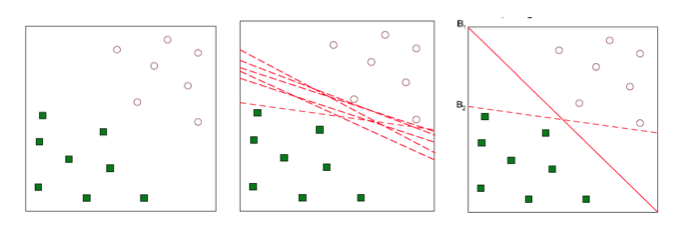
\includegraphics[width=.7\textwidth]{images/svm.png}
\caption{ Hiper-ravan u metodi podržavajućih vektora }
\label{img:svm_1}
\end{figure}

Na slici \ref{img:svm_1} prvo su prikazani podaci u dve klase.  Jedna klasa je predstavljena belim kužićima,  a druga klasa zelenim kvadratićima.  U srednjem delu su prikazane neke od mogućih hiper-ravni koje razdvajaju ova dva skupa.  Na desnom delu slike su predstavljene dve koje poredimo,  $B_1$ i $B_2$. Slika je preuzeta iz rada TODO cite Jelena.  Kako je cilj da hiper-ravan maksimizuje veličinu margine od nje do najbližih instanci oba skupa, možemo zaključiti da treba izabrati $B_1$. 

\begin{figure}[h!]
\centering
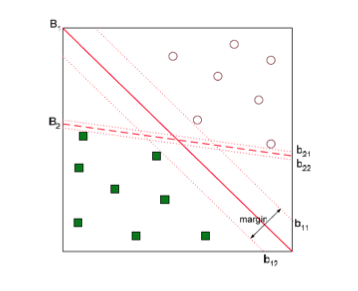
\includegraphics[width=.7\textwidth]{images/svm1.png}
\caption{ Hiper-ravan u metodi podržavajućih vektora sa marginom }
\label{img:svm_2}
\end{figure}
\noindent
Na slici \ref{img:svm_2} su grafički prikazane margine oko obe ravni i vidi se koja margina je veća. Slika je preuzeta iz rada TODO cite Jelena. 

Proces učenja kada se određuje optimalna hiper-ravan se radi, kao i u ostalim algoritmima klasifikacije, na skupu za treniranje.  Kada se radi korak predikcije, za svaku instancu se određuje rastojanje od te ravni i prema tome sa koje strane se nalazi, dodeljuje joj se jedna od klasa. 

Neka je dato \textit{n} objekata koje treba klasifikovati \textit{n\normalfont(x1,y1\normalfont),\normalfont($x_2$,$y_2$\normalfont),...,\normalfont($x_n$,$y_n$\normalfont)},  gde su $x_i \in R^n$ instance ,   $y_i \in \{-1,1\}$ predstavlja klasu kojoj instanca pripada.  Cilj je naći takvu hiper-ravan da razdvaja instance kojima je klasa $y$ = 1 i one kojima je $y$ = -1 i pretpostavimo da važi uslov linearne razdvojivosti:
Jednačina hiper-ravni se predstavlja izrazom:
\begin{equation}
	w\textsubscript{x}+w\textsubscript{0} = 0
\end{equation}
{\setlength{\parindent}{0cm}
gde je $w$ vektor težina i odrežuje smer hiper-ravni, a $w_0$ pomeraj.  Optimalna hiper-ravan je ona koja je maksimalno udaljena od najbližih predstavnika klasa.  Te dve instance koje su najbliže predstavljaju potporne vektore, a po njima je ova metoda i dobila ime. Jednačine dve ravni koje su paralelne sa optimalnom,  a prolaze kroz te najbliže predstavnike klasa su:
}
\begin{equation}
	w\textsubscript{x}+w\textsubscript{0} = c \\
\end{equation}
\begin{equation}
	w\textsubscript{x}+w\textsubscript{0} = -c
\end{equation}
{\setlength{\parindent}{0cm}
Kada podelimo sve jednačine sa c, za neke nove parametre $w_x$ i $w_0$ dobijamo sledeće jednačine:
}
\begin{equation}
	w\textsubscript{x}+w\textsubscript{0} = 0
\end{equation}
\begin{equation}
	w\textsubscript{x}+w\textsubscript{0} = 1
\end{equation}
\begin{equation}
	w\textsubscript{x}+w\textsubscript{0} = -1
\end{equation}
\noindent
Jednačina rastojanja tačke od hipe-ravni je sledeća:
\begin{equation}
	\frac{|w \cdot x + w\textsubscript{0}|}{\|w\|\textsubscript{2}}
\end{equation}
\noindent
pa tako dobijamo da je rastojanje između klasa u pravcu normalnom na optimalnu hiper-ravan sledeće:

\begin{equation}
	\frac{2}{\|w\|}
\end{equation}
\noindent
Pošto pokušavamo da maksimizujemo ovo rastojanje,  ako rešavamo optimizacioni problem minimizacijom, dobijamo sledeći izraz:

\begin{equation}
	\min_{w,w_0} \frac{\|w\textsubscript{2}\|}{2} \\
\end{equation}
\begin{equation}
	y\textsubscript{i}(w \cdot x\textsubscript{i} \geq 1) \text{ za i = } \overline{1,n}
\end{equation}
\noindent
Ovo predstavlja kvadratni optimizacioni problem uz linearne uslove koji se može rešiti uz pomoć Langranžovih množioca. 

\begin{equation}
	w = \sum \alpha\textsubscript{i}y\textsubscript{i}x\textsubscript{i}
\end{equation}
\noindent
gde su $\alpha\textsubscript{i}$ takvi da je $0 \geq \alpha\textsubscript{i} \geq C$. Potporni vektori su takve instance $x_i$ za koje važi da je $\alpha\textsubscript{i} \geq 0$. 
\noindent
Model je dat funkcijom:
\begin{equation}
	f\textsubscript{w, w\textsubscript{0}}(x) = \sum_{i=1}^{N} \alpha\textsubscript{i}y\textsubscript{i}(x\textsubscript{i} \cdot x\textsubscript{0})
\end{equation}
\noindent
gde je $w_0$ optimalna hiper-ravan.  Klasa za instancu se predviđa sledećim izrazom:
\begin{equation}
	sgn(f\textsubscript{w, w\textsubscript{0}}(x))
\end{equation}
\noindent
Treba naći prag odlučivanja $p$, takav da važi:
$f(x) $ > p, ako element pripada klasi, 
$f(x) $ < p, ako element ne pripada klasi, 
$f(x) $ ) p,  ako je nedefinisan slučaj. 
\noindent
Problem sa prethodnim izrazom predstavlja cinjenica da smo pretpostavili linearnu razdvojivost klasa.  Na stvarnom skupu podataka, neophodno je prihvatiti neke greske i tada problem rešavamo medtodom sa mekim pojasom ili pomoću kernela.

\subsection{Metod sa mekim pojasom}
Za metod sa mekim pojasom (eng. soft margin) uvodimo promenljive $\xi_i$ za $\overline{1,n}$ koje prikazuju koliko je instanca daleko od optimalne hiper-ravni ako je ona sa pogrešne strane.  Uvodi se i parametar C koji je nenegativan i kontroliše koliko težine se pridaje greškama. Ako je $C=0$, greške nisu važne,  a ako je C veliko, onda su greške važne a pravac hipderravni i širina pojasa.  Optimizacioni problem sada izgleda ovako:

\begin{equation}
	\min_{w,w_0} \frac{\|w\textsubscript{2}\|}{2} + C \sum_{i=1}^{N} \xi_\textsubscript{i} \notag\\
\end{equation}
\begin{equation}
	y\textsubscript{i}(w \cdot x\textsubscript{i} \geq 1 - \xi_\textsubscript{i}) \text{ za i = } \overline{1,n} \notag\\
\end{equation}
\begin{equation}
	\xi_\textsubscript{i} \geq 0 \text{ za i = } \overline{1,n}
\end{equation}

\subsection{Kerneli}



\chapter{Rezultati}



\chapter{Zaključak}



% ------------------------------------------------------------------------------
% ------------------------------------------------------------------------------

% ------------------------------------------------------------------------------

% ------------------------------------------------------------------------------
% 
% ------------------------------------------------------------------------------
%\literatura

\bibliographystyle{amsplain}
\bibliography{Master_rad}


% ==============================================================================
% Završni deo teze i prilozi
\backmatter
% ==============================================================================


% ------------------------------------------------------------------------------
% Biografija kandidata
\begin{biografija}
  \textbf{Ljubica Peleksić} (\emph{Beograd,
    18.  novembar 1993.}) 
	Ljubicina biografija
\end{biografija}
% ------------------------------------------------------------------------------


\end{document}